\documentclass{article} % For LaTeX2e
\usepackage{nips12submit_e,times}
%\documentstyle[nips12submit_09,times,art10]{article} % For LaTeX 2.09
\usepackage{amsmath}
\usepackage{amssymb}
\usepackage{amsthm}
\usepackage{algpseudocode}
\usepackage{algorithmicx}
\usepackage{algorithm}
\usepackage{graphicx}
\usepackage{natbib}

\title{Continuous Domain Reinforcement Learning using Rapidly-exploring Random Trees}


\author{
David S.~Hippocampus\thanks{ Use footnote for providing further information
about author (webpage, alternative address)---\emph{not} for acknowledging
funding agencies.} \\
Department of Computer Science\\
Cranberry-Lemon University\\
Pittsburgh, PA 15213 \\
\texttt{hippo@cs.cranberry-lemon.edu} \\
\And
Coauthor \\
Affiliation \\
Address \\
\texttt{email} \\
\AND
Coauthor \\
Affiliation \\
Address \\
\texttt{email} \\
\And
Coauthor \\
Affiliation \\
Address \\
\texttt{email} \\
\And
Coauthor \\
Affiliation \\
Address \\
\texttt{email} \\
(if needed)\\
}

% The \author macro works with any number of authors. There are two commands
% used to separate the names and addresses of multiple authors: \And and \AND.
%
% Using \And between authors leaves it to \LaTeX{} to determine where to break
% the lines. Using \AND forces a linebreak at that point. So, if \LaTeX{}
% puts 3 of 4 authors names on the first line, and the last on the second
% line, try using \AND instead of \And before the third author name.

\newcommand{\fix}{\marginpar{FIX}}
\newcommand{\new}{\marginpar{NEW}}

%\nipsfinalcopy % Uncomment for camera-ready version

\begin{document}


\maketitle

\begin{abstract}
The problem of efficient exploration for reinforcement learning is difficult, more so in domains that have continuous states and continuous actions. We present a novel algorithm based on Rapidly-exploring Random Trees to solve such problems.
\end{abstract}

\section{Introduction}
Reinforcement Learning(RL) deals with learning optimal control strategies through interactions with the world. One of the major hindrances in extending standard RL techniques to real world scenarios, is their inability to deal with continuous valued variables. Straightforward discretization of the space leads to several problems. The discretization might be too small or too large leading to large amounts of learning time needed or incorrect generalization correspondingly. Methods that use function approximators are also popular but they need to be fine tuned according to the domain. Least Squares Policy Iteration \cite{lspi} is a popular algorithm that uses linear function approximation and offline data from several trajectories in the space to learn the solution. However this offline data needs to be sufficiently representative to arrive at the correct solution.\\
 This leads us to another fundamental problem in reinforcement learning which is the problem of balancing exploration and exploitation. This becomes an even more daunting task in continuous domains as the amount of space to be explored can be huge. An algorithm that attempts to optimally balance explore-exploit is the UCT algorithm\cite{uct}. This however does not work in continuous spaces. In an attempt to make an online version of LSPI it has been combined with R-MAX, a technique that does efficient exploration in discrete domains\cite{rmaxlspi} . However this has several implementation issues such as tuning exploration parameters and generalizing state visitation counters. Often in such domains a model or simulator is available and several model based algorithms exist. One such approach is PEGASUS \cite{pegasus} which makes a large problem more feasible by using a model of the world.\\
 We tackle the problem of exploration in continuous space by making use of Rapidly-exploring Random Trees(RRTs), a widely popular sample-based planning techniques in the robotics\cite{rrt}. RRTs have several attractive properties that we exploit - they are parameter free and have provable exploration properties. We present an model based algorithm that solves continuous domain RL problems through an adaptive discretization of the space based on RRTs. This work is similar in spirit to the parti-game algorithm for adaptive discretization\cite{partigame}. However the splitting criterion for our algorithm is exploration centric. Our algorithm is motivated by the RRT*\cite{rrtstar} algorithm, which is an \emph{optimal} version of the RRTs. The algorithm which we present is an generalized version of the RRT* algorithm as applied to RL problems and tries to achieve optimal corresponding optimal solutions. Section 2 will introduce some preliminaries as well as explain the RRT and RRT* algorithms. Our algorithm RRT-VI will be described in Section 3, followed by discussions and experimental results.


\section{Preliminaries}
\label{sec:prelims}
A Markovian Decision Process(MDP) is described as $\left\langle S,A,P,R\right\rangle$, where $S\in \mathbb{R}^n$ is the domain of states and $A\in \mathbb{R}^m$ is the domain of actions. $P$ is the state transition probability. $R$ is a real valued reward function. The aim of the \textit{RL agent} is to maximize the discounted cumulative reward obtained.
A deterministic policy $\pi$ is a mapping from the state space $S$ to the action space $A$. $V^\pi(s)$ is the state value function and is equal to the expected long term rewards, by following $\pi$ at $s$. Similarly, $Q^\pi(s,a)$ is the state-action value function. The value function might be expressed as,
\begin{equation}
\label{eq:Vbell}
\forall s \in S,\;\; V^\pi(s) = R(s) + \gamma \sum_{s'}P^{ss'}_{\pi(s)}V^\pi(s')
\end{equation}
where $s'$ is the state transitioned to and $\gamma \in \left(0,1\right)$ is the discount factor. A policy $\pi^*$ is optimal if $ \forall s,\pi\;\; V^{\pi^*}(s)\geq V^\pi(s) $ The optimal value function can be calculated by replacing the expectation in Equation \ref{eq:Vbell} with $\max$. A similar set of equations exist for the $Q$ function.

\subsection{Rapidly-exploring Random Trees}
\label{sec:rrt}
\begin{figure}[htb]
% Caption and label go in the first argument and the figure contents
% go in the second argument
\centering
\label{fig:rrt}
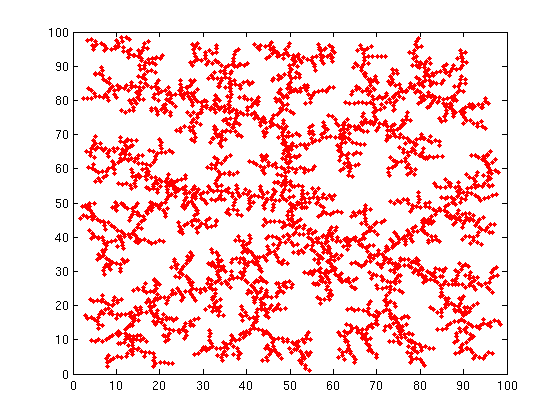
\includegraphics[scale=0.45]{rrt.png}
\caption{RRT with 300 nodes grown in $(0,100)^2$ starting from (50,50)}
\end{figure}

The basic RRT construction is outlined in algorithm \ref{alg:basicrrt}. The algorithm is straightforward and elegant.  Figure \ref{fig:rrt} shows a RRT grown in a 2 dimensional space. The algorithm builds a Tree $T$ of samples from some space $S$ whose nodes and edges are represented by $V(T)$ and $E(T)$. The tree is rooted from a given state $s_{start}$ and is grown as described. Extend the tree towards the closest point implies adding an new node in the direction of the sample point and connecting it with the nearest existing point on the tree.   RRTs have been shown to be \textit{asymptotically complete}\cite{rrtconnect}. 
\[ \lim_{\mid V(T)\mid \rightarrow \infty } Pr(s\in V(T)) \rightarrow 1\,\,, \forall s\in S \] 
RRTs can be thought of as monte-carlo versions space-filling trees. Given a tree $T$ the space $S$ can be split into $|V(T)|$ regions each corresponding the Voronoi region of the nodes. When a point is sampled uniformly in the space, it can be seen that the node to be expanded in the third step of the RRT algorithm is chosen with a probability proportional to the volume of its Voronoi region. This implicitly directs exploration towards unexplored parts of the state space. 
\begin{algorithm}
\caption{ConstructRRT}
\label{alg:basicrrt}
\begin{algorithmic}
\State $V(T)=s_{start},\,E(T)=\emptyset$
\Repeat 
	\State Uniformly sample a state $s$ from space $S$
	\State Calculate closest point in tree to $s$
	\State Extend the tree from the closest point towards $s$ 
\Until{termination}
\end{algorithmic}
\end{algorithm}

\subsection{RRT*}
RRT* is a variation of the standard RRT planner. It produces \emph{asymptotically optimal} solutions as well as giving \emph{asymptotically complete} guarantees of RRT\cite{rrtstar}. The algorithm is similar to the original RRT algorithm with an added step - it `rewires' the tree within some region as shown in steps 5-7 in Algorithm \ref{alg:rrtstar}. Thus reducing the path length from the root of the tree to the new point added to the tree. The neighborhood in which the rewiring is done is a hypersphere of radius = $O((log(|V(T)|)/|V(T)|)^{1/d})$ where d is the dimensionality of the space $S$. Thus as the tree grows, the size of sphere falls such that the number of possible connections at every step is in $O(log(|V(T)|))$. Hence the additional computational overhead is not significantly more than the original RRT algorithm. 
\begin{algorithm}
\caption{ConstructRRT}
\label{alg:rrtstar}
\begin{algorithmic}[1]
\State $V(T)=s_{start},\,E(T)=\emptyset$
\Repeat 
	\State $s_{new}\leftarrow $ Uniform random sample
	\State $s_{nearest}\leftarrow $ Choose nearest point in tree from $s_{new}$
	\State $s_{center}$ Choose point to extend $s_{nearest}$ towards $s_{new}$
	\State $S_{near}\leftarrow $ Select all points in the tree within some radius $r$ from $s_{center}$
	\State Connect the closest point in the set $S_{near}$ to $s_{center}$
\Until{termination}
\end{algorithmic}
\end{algorithm}
The actual radius $r$ in step 6 of the Algorithm \ref{alg:rrtstar} is $\gamma(log(|V(T)|)/|V(T)|)^{1/d}$ where $\gamma > 2(1+1/d)^{1/d}(\mu(S)/\zeta_d)^{1/d} $. $\mu(S)$ is the Lebesgue measure of the space $S$ and $\zeta_d$ is the volume of the d-dimensional unit ball. 
The RRT* algorithm produces asymptotically optimal paths to the goal region from some start point. In a similar manner, the our algorithm samples from the MDP and attempts to optimize trajectories w.r.t expected long term rewards i.e. the value function.

\section{RRT-VI}
\begin{enumerate}
\item A generative model $\mathcal{M}$ that allows us to sample the reward function given a state transition.
\item An \textit{approximate local controller} that can move from a given state to any state in its neighborhood. Note that this controller may not always move to the intended target state due to stochasticity in the state transitions.
\end{enumerate}

\section{Discussion} 

\section{Experimental Results}

\section{Conclusion and Future Work}

\bibliographystyle{unsrt}
\bibliography{rrtpi}

\end{document}
